%\documentclass[11pt]{article}
\documentclass[11pt]{IEEEtran}

\usepackage[utf8]{inputenc}
\usepackage[brazilian]{babel}

\usepackage{indentfirst}
\usepackage{xcolor}         % Permite o uso de cores no texto
\usepackage{colortbl}       % Permite colorir tabelas
\usepackage{amsmath}        % Permite escrever os conjuntos matemáticos
\usepackage{amssymb}        % Permite usar mais símbolos matemáticos, como o não existe.
\usepackage{amsfonts}
\usepackage{enumerate}      % Inclui a função enumerate 
\usepackage{graphicx}
\usepackage{hyperref}       % Permite o uso de hyperlinks no texto, com um link clicável
\usepackage{tikz}           % Permite criar imagens
\usepackage{multicol}       % Permite usar texto com várias colunas

\usepackage{pythonhighlight}

\usepackage[top=2cm, bottom=2cm, left=3cm, right=3cm]{geometry}

\renewcommand{\baselinestretch}{1.2}
\setlength\parindent{5.5mm}

\renewcommand{\b}[1]{\textbf{#1}} %Define um resumo de um comando
\newcommand{\blue}[1]{\textcolor{blue}{#1}}
\newcommand{\blueb}[1]{\textbf{\textcolor{blue}{#1}}}

\newcommand{\inn}{$\in \mathbb{N}$ \ } % Abreviação para "no conjunto dos naturais".
\newcommand{\inz}{$\in \mathbb{Z}$ \ } % Abreviação para "no conjunto dos inteiros".

\newcommand{\pontoI}{\begin{enumerate}[\indent $\bullet$]} % Cria o início da indentação normal do ponto
\newcommand{\tracoI}{\begin{enumerate}[\indent -]} % Cria o início da indentação normal do traço.

\newcommand{\fim}{\end{enumerate}} %Finaliza a indentação do ponto

\newcommand{\imp}{$\Rightarrow$ \ } % Cria a seta de implicação

\title{Compartilhamento de arquivos por FTP \\ \LARGE EzShare}
\author{Gabriel Henrique do Nascimento Neres - 221029140 \\ Guilherme Nonato da Silva - 221002020}

\begin{document}

\maketitle

\begin{abstract}
   O presente relatório visa 
\end{abstract}

% \begin{keywords}
%    FTP, .
% \end{keywords}


 \textbf{\textit{Palavras-chave — }FTP, Servidor, Python.} 

\section{Introdução}
% Contextualização do tema do trabalho dentro da disciplina e da área de redes de computadores. Descrição da estruturação do relatório.
% O tema do trabalho é a implementação de um cliente de um servidor FTP. A descrição da estrutura deve ser relacionada com a descrição das divisões dos capítulos e o que será tratada em cada uma

%- Explicar o intuito do trabalho
%- Citar as ferramentas utilizadas
%- Relacionar o trabalho com a disciplina
%- Explicar a estrutura do relatório

O intuito do trabalho a ser desenvolvido é compreender e implementar um cliente capaz de se comunicar com um servidor FTP, contando com uma interface que permita a um possível usuário utilizar o programa criado intuitivamente. Utilizaremos a versão 3.11 do Python para o desenvolvimento do código, tanto para configurar o cliente quanto para desenvolver a interface gráfica. Para o servidor será utilizado o servidor FTP já implementado por padrão no sistema operacional Windows.

O presente relatório se dividirá em mais três seções: 
\pontoI
\item Uma para situar o conteúdo teórico do projeto e contextualizar o material aprendido em aula; 
\item Uma focada em analisar e descrever as implementações feitas e os resultados obtidos pelo programa desenvolvido, sendo subdividido em três tópicos:
\tracoI
    \item Funcionalidades do cliente;
    \item Exemplos de uso do cliente com o fluxo de mensagem entre cliente e servidor;
    \item Análise da comunicação cliente-servidor pelo \textit{Wireshark} com a identificação dos endereços IP e a análise das mensagens para comprovar o bom funcionamento do cliente.
\fim
\item Uma última para extrair conclusões dos processos feitos, além de considerar o que foi aprendido ao decorrer do projeto.

\fim

\section{Fundamentação Teórica}
% Descrição dos conceitos teóricos e técnicas que foram utilizados e aplicados para desenvolver a compreensão do trabalho e o ambiente experimental.
% Conceitos teóricos que são importantes para o projeto:
% FTP: Definição do protocolo e funcionamento do servidor
% TCP: Definir o funcionamento da comunicação para a explicação da parte do WireShark.
% Princípio da transferência de dados.

O projeto da construção de um cliente para um servidor do tipo FTP necessitou do estudo e a compreensão de alguns dados teóricos. Dentre as informações utilizadas podem ser elencadas os conceitos ligados ao protocolo utilizado por um servidor FTP, o funcionamento de uma comunicação TCP e os princípios da transferência de dados.

O \b{protocolo FTP} \cite{FTP} define diversas instruções e funcionalidades baseado no protocolo do TELNET. Os principais conceitos que precisaram ser conhecidos para o desenvolvimento do cliente que iria se comunicar com o servidor foram:
\pontoI
   \item \b{Caminho de dados}: Para a transferência de dados entre o servidor e o cliente é preciso estabelecer um caminho de dados entre os dois. O caminho de dados é um canal que é criado para a transferência de um único "arquivo" entre o \textit{host} e o servidor, o que cria a necessidade de iniciar e finalizar a conexão de dados entre eles para cada solicitação feita.
   \item \b{Conexão Passiva e Ativa}: O conceito foi importante para determinar qual tipo de conexão deveria ser estabelecida pelo cliente para alcançar o objetivo desejado. Esse conceito está diretamente ligado com a criação do caminho de dados.
\fim


\section{Análise de Resultados}
No desenvolvimento do sistema que seria estudado foi necessária a implementação do servidor FTP. Em função da simplicidade para a configuração, o servidor FTP disponibilizado pelo sistema operacional Windows foi utilizado para ser o servidor a ser acessado pelo cliente desenvolvido.

O servidor não precisou de nenhuma configuração especial. Foram definidos o IP do servidor, que para facilitar a obtenção dos dados que serão utilizados posteriormente foi utilizado o 127.0.0.1 (Indicativo de rede local), a porta de acesso 21 (padrão do servidor FTP) e um usuário e senha para acessar o servidor. Dessa forma, são concluídas as configurações do servidor.

Na próxima parte da análise será definida como foi feita a implementação do cliente. Para isso, a explicação foi dividida em subseções para a obtenção de uma melhor organização dos pontos observados.

\subsection{Funcionalidades do cliente}
Na busca de um cliente que desempenhasse todos as ações desejadas, foram necessários diversos comandos FTPs que precisaram ser reunidos em "macro" funções que seriam capazes de realizar todas as comunicações básicas entre cliente e servidor.

A primeira funcionalidade implementada foi a de criação do socket para a realização da comunicação. Para isso será utilizada uma biblioteca padrão do Python chamada Socket \cite{socket}. O código para isso pode estar definido como:
\begin{python}
def criarSocket(host,port):   
    socket = s.socket(s.AF_INET, 
    s.SOCK_STREAM)
    endereco = (host, port)
    socket.connect(endereco)
    receberMensagem(socket) 
    return socket
\end{python}

Com o socket definido, pode ser feita a conexão e definição das configurações do servidor. Para isso será usado o usuário e senha criados e será definido o tipo de código ASCII utilizado.
\begin{python}
# Faz login no servidor
def Login(socket, user, senha):
    usuario = "user {u}\r\n"
    .format(u = user)
    comunicar(socket, usuario)# Login
    password = "pass {s}\r\n"
    .format(s = senha)
    comunicar(socket, password)# Senha

# Estabelece uma conexao com o 
# servidor (com login) e configura
def Conectar(Usuario, Senha):
   socket = criarSocket(host, port)
   Login(socket, Usuario, Senha)
   comunicar(socket,"opts UTF8 ON\r\n")
   return socket
\end{python}

Sendo assim estão definidas as funções de conectar e logar ao servidor a partir de um socket feito pelo cliente. As próximas funções a serem definidas são a de envio e recebimento de mensagens do servidor.

Envio: Manda a mensagem informada pelo socket.
\begin{python}
# Tenta enviar uma mensagem ao servidor
def mandarMensagem(socket, mensagem):
  try:
    socket.settimeout(0.2)
    socket.send(mensagem.
           encode('utf-8'))
  except:
    print("Time out")
\end{python}

Recebimento: Recebe todas as mensagens vindas pelo socket até que ocorra o \textit{timeout} durante alguma execução do loop.
\begin{python}
# Tenta recebe as mensagens do servidor
def receberMensagem(socket):
  TimeOut = False
  mensagemTotal = ""
  Vazio = 0
  # Recebe so servidor ate superar 
  #o limite de tempo
  while not TimeOut:
    try:
     socket.settimeout(0.2)
     resposta = socket.recv(2048)
     dados = resposta.decode('utf-8')
     if dados in ["","\n","\r","\r\n"]:
        Vazio += 1
        if Vazio >= 2:
          return mensagemTotal
     else:
       print(dados)
       mensagemTotal = mensagemTotal 
                            + dados
    except:
      TimeOut = True
  return mensagemTotal
\end{python}

Com essas funções, é possível realizar todo o tipo de interação com o servidor, mas para simplificar a implementação da interface do cliente foram construídas mais funções. Dentre as principais funções construídas está a responsável por iniciar um caminho de dados.
\begin{python} 
def caminhoDeDados(socket):
 mandarMensagem(socket, "pasv\r\n")
 dados = receberMensagem(socket)
 eliminar = ",.()\r\n"
 endereco = [item for item in dados
            .split(" ")[-1].split(",")]
 P1 = endereco[-2]
 P2 = "".join([caracter for caracter in 
    endereco[-1] if caracter not in 
                            eliminar])
 porta = int(P1)*256 + int(P2)
 caminho = s.socket(s.AF_INET, s.
                        SOCK_STREAM)
 end = (host, porta)
 caminho.connect(end)
 receberMensagem(caminho)
 return caminho
\end{python}

Neste trecho de código o comando PASV é enviado ao servidor para inciar uma conexão passiva com o mesmo. Utilizando o IP obtido dessa conexão, um novo socket é criado para a transmissão de dados e é retornado para a parte do código que solicitou esse socket. É importante ressaltar que o socket gerado só pode ser usado para uma única comunicação troca de dados com o servidor.

Utilizando tudo que foi construído até agora, é possível construir funções que utilizem retornos do caminho de dados. Em todas elas, o comando será enviada ao servidor pelo socket inicial após a criação do caminho de dados e a resposta esperada será obtida pelo socket do caminho de dados. As respostas obtidas pelo socket normal são usadas para garantir que a transição ocorreu como o esperado.

A primeira destas implementações é uma função que retorne tudo que está em um determinado diretório do servidor.

\begin{python}
#Lista os objetos no caminho indicado
def Listar(socket, path):
 caminho = caminhoDeDados(socket)
 mensagem = "list "+path+final
 mandarMensagem(socket, mensagem)
 confirmacao = receberMensagem(socket)
 conteudo = receberMensagem(caminho)
 receberMensagem(socket)
 caminho.close()
 return confirmacao, conteudo
\end{python}

A próxima função solicita um arquivo do servidor e cria uma cópia no cliente em um diretório especificado.
\begin{python}
def Download(socket, pathS, pathL):
 caminho = caminhoDeDados(socket)
 mensagem = "RETR "+pathS+final
 mandarMensagem(socket, mensagem)
 confirmacao = receberMensagem(socket)
 conteudo = receberMensagem(caminho)
 receberMensagem(socket)
 caminho.close()
 criarArquivo(pathL, conteudo) 
 return confirmacao

def criarArquivo(pathL, conteudo):
 try:
  if type(pathL) == type(["lista", "de"
                           , "teste"]):
   path = "".join(x+" " for x in pathL)
   with open(file=path, mode = "x") 
                                 as f:
      f.write(conteudo)
  else:
   with open(pathL, "x") as f:
      f.write(conteudo)
 except FileNotFoundError:
    print("O path tem problemas")
 except FileExistsError:
    print("Arquivo com o mesmo nome")
\end{python}

De maneira similar é possível enviar um arquivo de um diretório específico do cliente ao servidor.
\begin{python}
def Upload(socket, pathS, pathL):
  caminho = caminhoDeDados(socket)
  path = "".join(x+" " for x in pathS)
  mensagem = "STOR "+path+final 
  texto = mandarArquivo(caminho, pathL)
  mandarMensagem(socket, mensagem)
  confirmacao = receberMensagem(socket)
  conteudo = receberMensagem(caminho)
  receberMensagem(socket)
  caminho.close()    
  return confirmacao

def mandarArquivo(socket, L):
 try:
   if type(pathL) == type(["lista"]):
    p = "".join(x+" " for x in L)
    mandarMensagem(socket, lerArq(p))
   else:
    mandarMensagem(socket,lerArq(L))
 except FileNotFoundError:
   print("Path tem problemas")
 except FileExistsError:
    print("Arquivo com o mesmo nome")

def lerArq(pathLocal):
  with open(pathLocal, "r") as f:
     tc = f.readlines()
     string = "".join([x for x in tc])
     return string
\end{python}

Dessa forma, são apresentadas todas as funções que foram implementadas no cliente.

\subsection{Exemplos de uso do cliente}
Para exemplificar o funcionamento do cliente, podem ser observados dois processos de comunicação com o servidor. No primeiro processo, o cliente apenas estabelece a conexão com o servidor para deixá-lo disponível para poder enviar e receber arquivos posteriormente.

% Tela com o servidor desconectado
\begin{figure}[h]
   \centering
   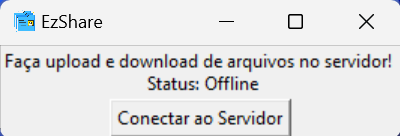
\includegraphics[width = 0.8\linewidth]{TelaNaoConectado.png}  
   \caption{Tela com o servidor desconectado.}
   \label{fig:Tela inicial}
\end{figure}


Ao clicar no botão de "Conectar ao Servidor" o cliente inicia uma série de comandos ao servidor. Primeiramente, é enviada uma mensagem TCP do cliente ao servidor para iniciar o HandShaking. Com o recebimento da resposta do servidor e o envio da confirmação por parte do cliente. Com isso é dado início os processos diretamente ligados ao protocolo FTP.

O usuário do login é enviado ao servidor, e a resposta obtida é o pedido de uma senha. Enviando a senha é obtida a confirmação da conexão com o servidor e permitindo a troca de informações internas do servidor. A última configuração realizada na conexão com o servidor é a definição do tipo de ASCII utilizado como UTF8.

\begin{figure}[h]
   \centering
   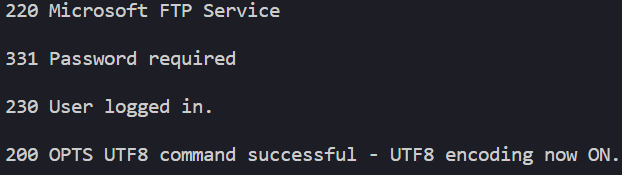
\includegraphics[width = 0.9\linewidth]{RespostasConexao.png}  
   \caption{Respostas do servidor.}
   \label{fig:Respostas do servidor}
\end{figure}

O segundo processo que pode ser observado é feito após a conexão com o servidor. Como inicialmente o servidor se encontrará vazio, o cliente desejará transferir algum arquivo ao servidor. Partindo dessa ideia, o processo pode ser descrito abstraindo a parte referente a conexão com o servidor. 

\subsection{\textit{WireShark}}
\section{Conclusões}
% Deve ter entre 5 e 10 linhas resumindo as conclusões obtidas com o trabalho.
 
% Verificar a formatação das referências
\begin{thebibliography}{10}
   \bibitem[1]{tkinter}{tkinter — Python interface to Tcl/Tk, \href{https://docs.python.org/3/library/tkinter.html}{https://docs. python.org/3/library/tkinter.html}}
   \bibitem[2]{socket}{socket — Low-level networking interface, \href{https://docs.python.org/3/library/socket.html}{https://docs .python.org/3/library/socket.html}}
   \bibitem[3]{FTP}{J. Postel, J. Reynolds. \textit{FILE TRANSFER PROTOCOL}, \href{https://www.rfc-editor.org/rfc/rfc959}{https://www.rfc-editor.org/rfc/rfc959}}
   \bibitem[4]{Comandos FTP}{J. Klensin, A. Hoenes. \textit{FTP Command and Extension Registry}, \href{https://www.rfc-editor.org/rfc/rfc5797}{https://www.rfc-editor.org/rfc/rfc5797}}
\end{thebibliography}


\end{document}